\documentclass{article}
\usepackage[utf8]{inputenc}
\usepackage{amsmath}
\usepackage{amssymb}
\usepackage{amsthm}
\usepackage{mathtools}
\usepackage[margin=1.0in]{geometry}

\title{COMP550 Notes}
\author{Chany Ahn}
\date{September 2021 - December 2021}

\begin{document}

\maketitle
\newpage
\tableofcontents
\newpage
\section{NLP and CL}
\subsection{Domains of Language}
\begin{itemize}
    \item \textbf{Phonetics}: Study of speech sounds that make up language.
    \item \textbf{Phonology}: Study of rules that govern sound patterns and how they're organized.
    \item \textbf{Morphology}: Word formation and meaning.
    \item \textbf{Syntax}: Study of the structure of language.
    \item \textbf{Semantics}: Study of the meaning of language.
    \item \textbf{Pragmatics}: Study of the meaning of language in context.
    \begin{itemize}
        \item \textbf{Deixis}: Interpretation of expressions can depend on extralinguistic context.
    \end{itemize}
    \item \textbf{Discourse}: Study of the structure of larger spans of language.
\end{itemize}

\section{Text Classification}
\subsection{Feature Extraction}
\begin{itemize}
    \item An input can be represented as a vector, $\vec{x}$, where the feature inputs can be binary: whether or no the word is in a given piece of text.
    \item \textbf{Lemma}: Removes affixes and recovers the lemma (form that you look up in the dictionary).
    \begin{itemize}
        \item Achieved using finite state automata.
    \end{itemize}
    \item \textbf{Stemming}: Cuts affixes to find the stem.
    \begin{itemize}
        \item Porter stemming: An ordered list of of rewrite rules to approximately recover the stem of a word.
        
        The basic idea is to chop off and append endings back onto a word.
    \end{itemize}
\end{itemize}
\subsubsection{N-Grams}
Sequences of \textit{adjacent words}. Version of N-Grams are:
\begin{itemize}
    \item Prescence or abscence of N-grams (0 or 1).
    \item Count of an N-gram.
    \item Proportion of the total document.
    \item Scaled versions of counts (ex. give common word lower weights and uncommon words larger weights).
\end{itemize}
\subsubsection{POS Tags}
Sequence of POS tags crudely captures syntatic patterns in text. The document must be pre-processed for their POS tags.
\subsubsection{Stop Words}
Common words may not be useful for some document classification tasks (highly task-dependent). Standardized list of such stop words are commonly removed.

\section{Linear Classifiers}
\subsection{Type/Token Distinction}
\begin{itemize}
    \item \textbf{Type}: the identity of a word (i.e., count unique words).
    \item \textbf{Token}: an instance of a word (i.e., each occurrence is separate).
\end{itemize}
Text classifications usually deals with tokens and assumes a categorical distribution that is used to generate all of the tokens seen in a sample, conditioned on class $y$.
\begin{itemize}
    \item Example: \textit{yo buy my stuff yo}, class: \textit{spam}.
    \[P(spam)P(yo|spam)P(my|spam)P(\textit{stuff}|spam)P(yo|spam)\]
\end{itemize}
\subsection{Generative vs. Discriminative}
\begin{itemize}
    \item \textbf{Generative} models learn a distribution for all random variables involved: joint distribution, $P(\vec{x},y)$.
    \item \textbf{Discriminative} models directly parameterize and learn $P(y|\vec{x})$ (better for text classification).
\end{itemize}

\subsection{Naive Bayes}
A probabilistic classifier that uses Bayes rule:
\begin{align}
    P(y | \vec{x}) = \frac{P(y)P(\vec{x}|y)}{P(\vec{x})}
\end{align}
Naive Bayes is a generative model:
\begin{itemize}
    \item Probabilistic account of the data $P(\vec{x},y)$.
    \item Naive Bayes assumes the dataset is generated in the following way, for each sample:
    \begin{enumerate}
        \item Generate label by $P(y)$.
        \item Generate feature vector $\vec{x}$ by generating each feature independently, conditioned on $y$: $P(x_i | y)$.
    \end{enumerate}
\end{itemize}
So, the Naive Bayes assumption is:
\begin{align}
    P(\vec{x}, y) = P(y) \prod_i P(x_i | y)
\end{align}
\subsubsection{Naive Bayes Model Parameters}
The parameters to the model, $\theta$, consist of:
\begin{itemize}
    \item Parameters of prior class distribution $P(y)$.
    \item Parameters of each feature's distribution conditioned on class $P(x_i | y)$.
\end{itemize}
With discrete data, we assume that the distributions $P(y)$ and $P(x_i | y)$ are categorical distributions.
\subsubsection{Training}
\textbf{Objective}: pick $\theta$ to mazimize the likelihood of the training corpus, $\mathcal{D}$:
\begin{align}
    L^{NB}(\theta) &= \prod_{(\vec{x},y) \in \mathcal{D}}P(\vec{x}, y; \theta)\\
    &= \prod_{(\vec{x},y) \in \mathcal{D}}P(y) \prod_i P(x_i | y)
\end{align}
This boils down to computing \textit{relative frequencies}:
\begin{itemize}
    \item $P(Y = y)$ should be set to proportion of samples that are within class $y$.
    \item $P(X_i = x | Y = y)$ should be set to proportion of samples with feature value $x$ among samples of class $y$.
\end{itemize}
\subsubsection{Inference}
After training, we would like to classify a new instance (i.e., we want $P(y | \vec{x})$). This is easy to get from $P(\vec{x}, y)$:
\begin{align}
    P(y | \vec{x}) &= \frac{P(\vec{x}, y)}{P(\vec{x})}\\
    &= \frac{P(y)\prod_i P(x_i|y)}{P(\vec{x})}
\end{align}
Calculate $P(\vec{x})$ marginalize over random variable $y$ by summing up numerator for all possible classes (Law of Total Probability).

\subsection{Logistic Regression}
Logit function (a.k.a., maximum entropy or MaxEnt classifier):
\begin{align}
    P(y|\vec{x}) = \frac{1}{Z}e^{a_1x_1 + a_2x_2 + \ldots + a_nx_n + b}
\end{align}
Gives continuous values in the interval $[0,1]$, where $Z$ is a normalizing constant to insure that it is a probability distribution. Typically used for classification problems (not really a regression model).
\subsubsection{Logistic Function}
Graphically, the function is as follows:
\begin{itemize}
    \item y-axis: $P(y|\vec{x}) = \frac{1}{Z}e^{a_1x_1 + a_2x_2 + \ldots + a_nx_n + b}$
    \item x-axis: $a_1x_1 + a_2x_2 + \ldots + a_nx_n + b$
\end{itemize}
\subsubsection{Features}
Features depend on both the document and the proposed class.
\subsubsection{Parameters in Logistic Regression}
\begin{align}
    P(y|\vec{x}) &= \frac{1}{Z}e^{a_1x_1 + a_2x_2 + \ldots + a_nx_n + b}\\
    \text{where } \theta &= \{a_1,a_2, \ldots, a_n, b\}
\end{align}
Learning means to maximize the conditional likelihood of the training corpus.
\begin{align}
    L^{LR}(\theta) &= \prod_{(\vec{x},y) \in \mathcal{D}}P(y|\vec{x}; \theta)\\
    \log L^{LR}(\theta) &= \sum_{(\vec{x},y) \in \mathcal{D}}\log P(y|\vec{x}; \theta)
\end{align}
\subsubsection{Optimizing the Objective}
We want to maximize:
\begin{align}
    \log L^{LR}(\theta) &= \sum_{(\vec{x},y) \in \mathcal{D}}\log P(y|\vec{x}; \theta)\\
    &= \sum_{(\vec{x},y) \in \mathcal{D}}\log \left(\frac{1}{Z}e^{a_1x_1 + a_2x_2 + \ldots + a_nx_n + b}\right)\\
    &= \sum_{(\vec{x},y) \in \mathcal{D}}\left(\sum_i a_ix_i - \log Z\right)
\end{align}
which is done using \textbf{gradient descent}.
\subsection{Support Vector Machines}
Let $\vec{x} \in \mathbb{R}^d$. A SVM learns a decision boundary as a line (or a hyperplane when there are $>2$ features).
\subsubsection{Margin}
The hyperplane is chosen to maximize the margin to the nearest sample in each class. This method also deals with the fact that the samples \textit{may not be linearly separable}.
\begin{center}
    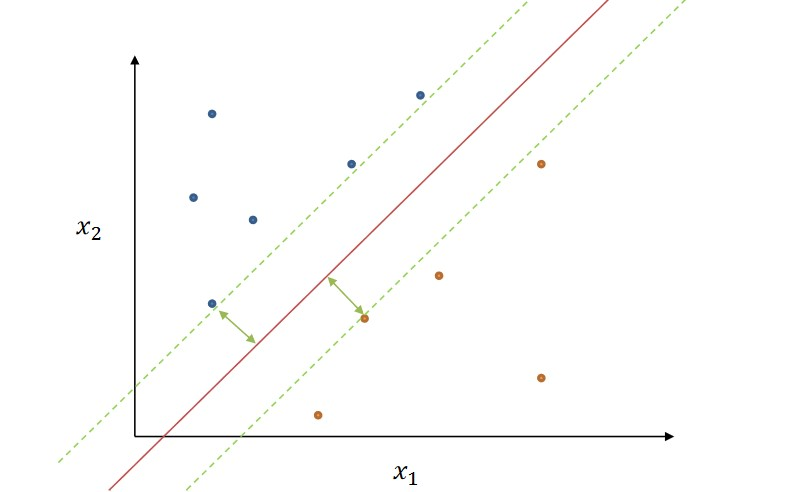
\includegraphics[scale = 0.75]{svm_boundary.jpg}
\end{center}
\subsection{Perceptron}
Closely related to logistic regression (differences in training and output interpretation):
\begin{align}
    f(\vec{x}) = \begin{cases}
    1 & \text{if } \vec{w} \cdot \vec{x} + b > 0\\
    0 & \text{otherwise}
    \end{cases}
\end{align}
\subsubsection{Stacked Perceptrons}
\begin{center}
    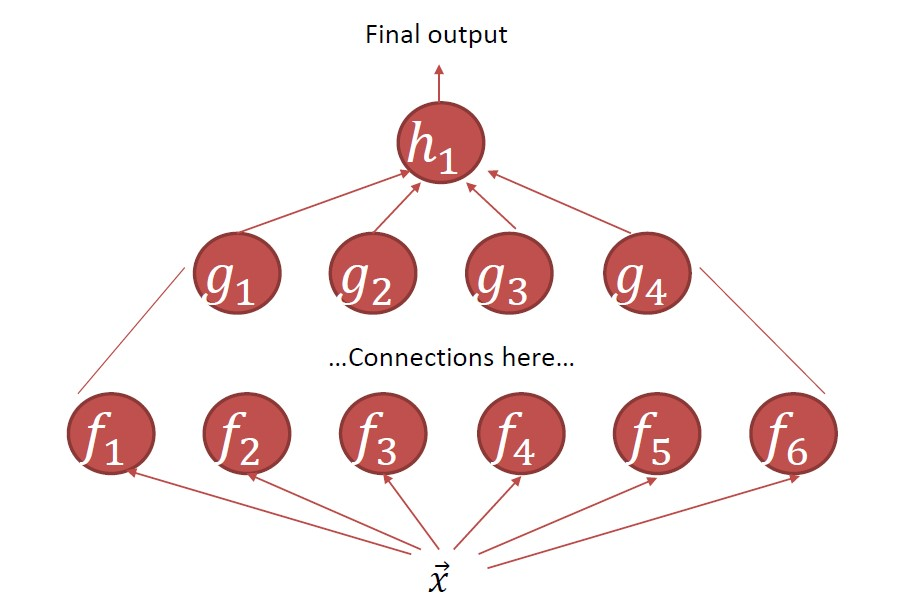
\includegraphics[scale=0.5]{stacked_percepton.jpg}
\end{center}
\subsection{Artificial Neural Networks}
Above is an example of an artificial neural network:
\begin{itemize}
    \item Each unit is a neuron with many inputs and one output.
    \item The nucleus fires given input from other neurons.
    \item Learning occurs at the synapses that connect neurons, either by amplifying or attenuating signals.
\end{itemize}
Advantages:
\begin{itemize}
    \item Can learn very complex functions.
    \item Many possible different network structures possible.
    \item Given enough training data, are currently achieving the best results in many NLP tasks.
\end{itemize}
Disadvantages:
\begin{itemize}
    \item Training takes a long time.
    \item Often need a lot of training data to work well.
\end{itemize}
\subsection{Other Classification Algorithms}
\begin{itemize}
    \item KNN
    \item Decision trees
    \item Transformation-based learning
    \item Random forests
\end{itemize}
\section{Nonlinear Classifiers}
Linear models cannot learn comlpex, non-linear functions from input features to output labels (without adding features).
\begin{itemize}
    \item Ex: Starts with a capital AND not at beginning of a sentence $\rightarrow$ proper noun (this is tough to represent with a linear model).
\end{itemize}
\subsection{(Artificial) Neural Network}
A kind of learning model which automatically learns non-linear functions from input to output. From the biologically inspired metaphor:
\begin{itemize}
    \item Network of computational units called neurons.
    \item Each neuron takes scalar inputs and produces a scalar output. This is similar to a logistic regression model:
    \[Neuron(\vec{x}) = g(a_1x_1 + \ldots + a_nx_n + b)\]
\end{itemize}
The network can, theoretically, compute any computable function, given enough neurons.
\subsection{Feedforward Neural Networks}
All connections flow forward (no loops); each layer of hidden units is fully connected to the next.
\begin{center}
    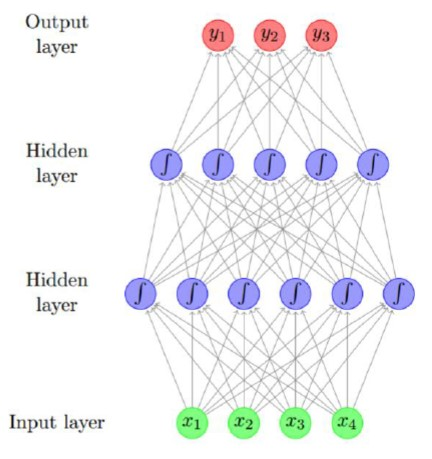
\includegraphics[scale=0.5]{feedforward_nn.jpg}
\end{center}
\subsubsection{Inference in a FF Neural Network}
Perform computations forwards through the graph:
\begin{align}
    \mathbf{h^1} &= g^1(\mathbf{xW^1} + \mathbf{b^1})\\
    \mathbf{h^2} &= g^2(\mathbf{xW^2} + \mathbf{b^2})\\
    \mathbf{y} &= \mathbf{h^2W^3}
\end{align}
Note, each layer is represented as a vector; combining all the weights in a layer across the units into a weight matrix.
\subsubsection{Activation Function}
In one unit: \textit{Linear comination of inputs and weight values $\rightarrow$ non-linearity}.
\[\mathbf{h^1} = g^1(\mathbf{xW^1} + \mathbf{b^1})\]
Some popular choices:
\begin{itemize}
    \item Sigmoid function
    \item $\tanh$ function
    \item Rectifier/ramp function: $g(x) = \max(0,x)$
\end{itemize}
Why is non-linearity important?
\subsection{Softmax Function}
In NLP, we often care about discrete outcomes. Output layer can be constructed such that the output values sum to one: let $\mathbf{x} = x_1\ldots x_k$.
\begin{align}
    softmax(x_i) = \frac{exp(x_i)}{\sum_j^k exp(x_j)}
\end{align}
\underline{Interpretation}: unit $x_i$ represents probability that outcome is $i$. Essentially, the last layer is like a multinomial logistic regression.
\subsection{Loss Function}
A neural network is optimized with respect to a \textit{loss function} which measures how much error it is making on predictions:
\begin{itemize}
    \item $\mathbf{y}$: correct, gold-standard distribution over class labels.
    \item $\mathbf{\hat{y}}$: system predicted distribution over class labels.
    \item $L(\mathbf{y},\mathbf{\hat{y}})$: loss function between the two.
\end{itemize}
A popular choice for classification is \textit{cross entropy} (especially with a softmax output layer):
\begin{align}
    L_{ce}(\mathbf{y},\mathbf{\hat{y}}) &= -\sum_i y_i\log(\hat{y}_i)
\end{align}
\subsection{Training Neural Networks}
Typically done by \textit{gradient descent}, we find the gradient of the loss function wrt parameters of the network (i.e., the weights of each layer). Since the network can have a lot of parameters, we use \textit{back-propagation} which is an efficient algorithm to compute the gradient wrt to all parameters. 

This boils down to an efficient way to use the chain rule of derivatives to propagate the error signal from the loss function backwards through the network back to the inputs.
\subsubsection{Gradient Descent}
Descent vs. Ascent: The convention is to think about the problem as a minimization problem. As stated before, we must minimize the loss function
\begin{align}
    \theta \leftarrow \theta - \gamma(\nabla L(\theta))
\end{align}
We do this by first initializing $\theta = \{\theta_1, \theta_2, \ldots, \theta_k\}$ randomly. The do the following algorithm for a while:
\begin{itemize}
    \item Compute $\nabla L(\theta)$ (through calculus)
    \item $\theta \leftarrow \theta - \gamma(\nabla L(\theta))$
\end{itemize}
Note: the gradient descent algorithm is computed over the entire training corpus.
\begin{itemize}
    \item Sum over all samples in training corpus.
    \item Weight update \textit{once} per iteration through the training corpus.
\end{itemize}
\subsubsection{Stochastic Gradient Descent}
SGD calculates the gradient over a small mini-batch of the training corpus and updates the weights. If the mini-batch size is one:
\begin{itemize}
    \item Many weight updates per iteration through the training corpus.
    \item Usually results in much faster convergence to final solution, without loss in performance.
\end{itemize}
\textbf{Overview}:
\begin{itemize}
    \item Inputs:
    \begin{itemize}
        \item Function computed by neural network: $f(\mathbf{x}; \theta)$.
        \item Training samples: $\{\mathbf{x}^k,\mathbf{y}^k\}$
        \item Loss function: $L$
    \end{itemize}
    \item Algorithm: Repeat for a while
    \begin{itemize}
        \item Sample of training cases: $\{\mathbf{x}^k,\mathbf{y}^k\}$
        \item Compute loss: $L(f(\mathbf{x}^k; \theta), \mathbf{y}^k)$ (forward pass).
        \item Compute gradient $\nabla L(\mathbf{x}^k)$ wrt the parameters $\theta$ (In neural networks, use backpropagation).
        \item Update $\theta \leftarrow \theta - \gamma(\nabla L(\theta))$
    \end{itemize}
\end{itemize}
\textbf{Example}:\\
Forward Pass
\begin{align*}
    \mathbf{h^1} &= g^1(\mathbf{xW^1} + \mathbf{b^1})\\
    \mathbf{h^2} &= g^2(\mathbf{xW^2} + \mathbf{b^2})\\
    f(\mathbf{x}) &= \mathbf{y} = g^3(\mathbf{h^2}) = \mathbf{h^2W^3}
\end{align*}
Loss function: $L(\mathbf{y},\mathbf{y}^{gold})$. Remember that we must save the values for $\mathbf{h^1}, \mathbf{h^2}, \mathbf{y}$.\\
Backpropagation
\[f(\mathbf{x}) = g^3(g^2(g^1(\mathbf{x})))\]
Need to compute: $\frac{\partial L}{\partial \mathbf{W}^3}, \frac{\partial L}{\partial \mathbf{W}^2}, \frac{\partial L}{\partial \mathbf{W}}$. By calculus and chain rule:
\begin{itemize}
    \item $\frac{\partial L}{\partial \mathbf{W}^3} = \frac{\partial L}{\partial g^3}\frac{\partial g^3}{\partial \mathbf{W}^3}$
    \item $\frac{\partial L}{\partial \mathbf{W}^2} = \frac{\partial L}{\partial g^3}\frac{\partial g^3}{\partial g^2}\frac{\partial g^2}{\partial \mathbf{W}^2}$
    \item $\frac{\partial L}{\partial \mathbf{W}} = \frac{\partial L}{\partial g^3}\frac{\partial g^3}{\partial g^2}\frac{\partial g^2}{\partial g}\frac{\partial g}{\partial \mathbf{W}}$
\end{itemize}
\subsection{Word Representations}
Previous word representations created vectors that held counts for each word found in the corpus: $[w_1\ w_2\ w_3\ w_4] = [\text{count}_1\ \text{count}_2\ \text{count}_3\ \text{count}_4]$.
\bigbreak \noindent
A more typical choice is to associate each word type with a fixed-dimensional vector which are model parameters: (don't really get this part)
\begin{align*}
    w_1&\ [0.3, 0.5, 0.6]\\
    w_2&\ [-0.1,0.2,0.7]
\end{align*}
\subsection{Sentence Representations}
To represent an input sentence or document, need to combine the input word vector representations:
\begin{itemize}
    \item Simple vector addition:
    
    this is a sentence $\rightarrow$ $v^{\text{this}}$ $v^{\text{is}}$ $v^{\text{a}}$ $v^{\text{sentence}}$ (look-up layer)
    
    $s = v^{\text{this}} + v^{\text{is}} + v^{\text{a}} + v^{\text{sentence}}$
    \item Component-wise vector multiplication
    
    $s = v^{\text{this}} \odot v^{\text{is}} \odot v^{\text{a}} \odot v^{\text{sentence}}$
\end{itemize}
There a many, sophisticated possible options.
\subsection{Hardware For NN}
Common operations in inference and learning:
\begin{itemize}
    \item Matrix multiplication
    \item Component-wise operations (e.g., activation functions)
\end{itemize}
These operations are highly parallelizable. Graphical processing units (GPUs) are specifically designed to perform this type of computation efficiently.
\subsection{Summary}
Advantages:
\begin{itemize}
    \item Learn relationships between inputs and outputs.
    \begin{itemize}
        \item Complex features and dependencies between inputs and states over long ranges with no fixed horizon assumptions (i.e., non-Markovian).
        \item Reduces need for feature engineering.
        \item More efficient use of input data via weight sharing.
    \end{itemize}
    \item Highly flexible, generic architecture.
    \begin{itemize}
        \item \textbf{Multi-task learning}: jointly train model that solves multiple tasks simultaneously.
        \item \textbf{Transfer learning}: Take part of a neural network used for an initial task, use that as an initialization for a second, related task.
    \end{itemize}
\end{itemize}
Challenges: complex models may need a lot of training data. There are many fiddly hyperparameters to tune, little guidance on how to do so, except empirically or through experience:
\begin{itemize}
    \item Learning rate, number of hidden units, number of hidden layers, how to connect units, non-linearity, loss function, how to sample data, training procedure, etc.
\end{itemize}
It can be difficult to interpret the output of a system.
\begin{itemize}
    \item Why did the model predict a certain label? We would have to examine weights in the network.
    \item Important to convince people to act on the outputs of the model!
\end{itemize}
\subsection{NNs for NLP}
NN have taken over mainstream NLP, and most empirical work at recent conferences use them in some way. Some interesting research questions:
\begin{itemize}
    \item How to use linguistic structure (e.g., word senses, parses, other resources) with NNs, either as input or output?
    \item When is linguistic feature engineering a good idea, rather than just throwing more data with a simple representation for the NN to learn the features?
    \item Multitask and transfer for NLP.
    \item Defining and solving new, challenging NLP tasks.
\end{itemize}
\subsection{Evaluation Measures}
To measure the performance of your classifier, the simplest option is \textbf{accuracy}:
\begin{align}
    \frac{\# \text{ correct}}{\# \text{ samples in test set}}
\end{align}
This is not always good. Consider the following case: Suppose that only one of every twenty emails is a \textit{spam} email. What would the accuracy of the classifier that always predicts \textit{non-spam} be? (What's the answer?)
\subsubsection{Precision and Recall}
\begin{align}
    \textbf{Precision} &= \frac{\# \text{ correct}}{\# \text{ predicted}}\\
    \textbf{Recall} &= \frac{\# \text{ correct}}{\# \text{ of that class}}
\end{align}
\subsubsection{Combining Precision and Recall}
$F1$ is the harmonic mean of precision and recall:
\begin{align}
    F1 = \frac{2 * P * R}{(P + R)}
\end{align}
Can combine $P$, $R$, $F1$ for each class:
\begin{itemize}
    \item \textbf{Macro-average}: take the average after computing $P$, $R$, $F1$ for each class.
    \begin{itemize}
        \item Weights each class equally. Good if all classes are equally important
    \end{itemize}
    \item \textbf{Micro-average}: take the sum of the counts first, then compute $P$, $R$, $F1$.
    \begin{itemize}
        \item Weights each sample equally.
    \end{itemize}
\end{itemize}
\subsection{Confusion Matrix}
It is often helpful to visualize the performance of a classifier using aconfusion matrix (horizontal represents the predicted class, and vertical represents the actual class):
\begin{center}
\begin{tabular}{|c|c|c|c|c|}
     \hline
     & $C_1$ & $C_2$ & $C_3$ & $C_4$\\
     \hline
     $C_1$ & count & count & count & count\\
     \hline
     $C_2$ & count & count & count & count\\
     \hline
     $C_3$ & count & count & count & count\\
     \hline
     $C_4$ & count & count & count & count\\
     \hline
\end{tabular}
\end{center}
We prefer if most of the cases fall into the diagonal entries.
\section{N-Grams}

\end{document}
